\section{Results}
\label{sec:results}

We test the four proposed dispatching strategies in the Zurich scenario.  Dispatching stages of all algorithms are called once every 30 seconds in simulated time, while the rebalancing periods for the AU and FF algorithms are 5 minutes. Those values have been obtained from prior simulation runs and could be subject to further optimization in future research. The simulation itself is performed on a per-second basis.


\subsection{Wait Times}
\label{sec:cost_analysis}

\begin{figure}
\centering
\begin{subfigure}{0.5\textwidth}
  \centering
  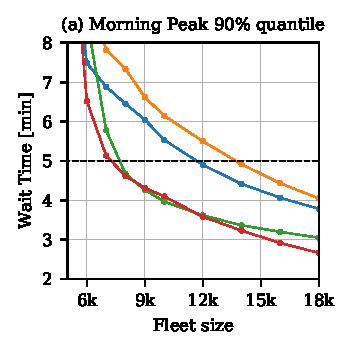
\includegraphics[width=2.35in]{figures/revision/rev_waiting_time_q90.pdf}
  %\caption{}
  %\label{fig:waiting_time_q90}
\end{subfigure}%
\begin{subfigure}{0.5\textwidth}
  \centering
  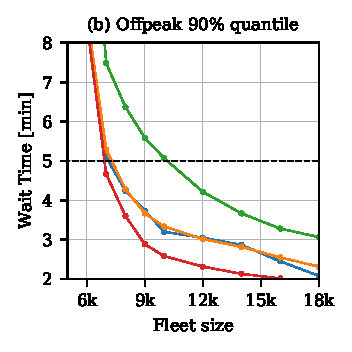
\includegraphics[width=2.35in]{figures/revision/rev_waiting_time_q90_offpeak.pdf}
  %\caption{}
  %\label{fig:waiting_time_q90}
\end{subfigure}
\begin{subfigure}{0.5\textwidth}
  \centering
  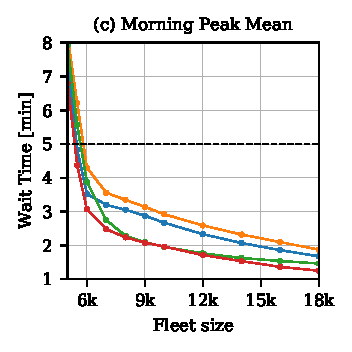
\includegraphics[width=2.35in]{figures/revision/rev_waiting_time_mean.pdf}
  %\caption{}
  %\label{fig:waiting_time_mean}
\end{subfigure}%
\begin{subfigure}{0.5\textwidth}
  \centering
  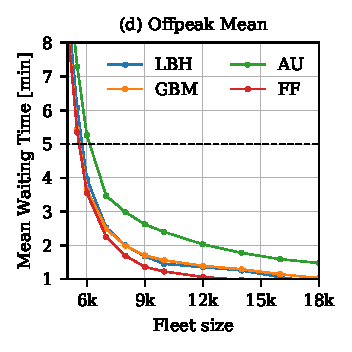
\includegraphics[width=2.35in]{figures/revision/rev_waiting_time_mean_offpeak.pdf}
  %\caption{}
  %\label{fig:waiting_time_mean}
\end{subfigure}
\caption{Comparison of morning peak (left) and off-peak (right) wait times generated by different operational policies. On top, the 90\% quantile is displayed, while
bottom row shows measured mean wait times.}
\label{fig:wait_time}
\end{figure}

%\begin{figure}
%\centering
%\begin{subfigure}{0.5\textwidth}
%  \centering
%  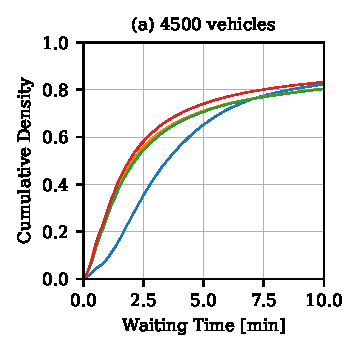
\includegraphics[width=2.35in]{figures/revision/rev_waiting_time_dist_4500.pdf}
%  \caption{}
%  \label{fig:waiting_time_dist_small}
%\end{subfigure}%
%\begin{subfigure}{0.5\textwidth}
%  \centering
%  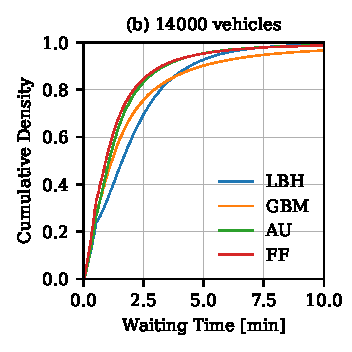
\includegraphics[width=2.35in]{figures/revision/rev_waiting_time_dist_14000.pdf}
%  \caption{}
%  \label{fig:waiting_time_dist_large}
%\end{subfigure}
%\caption{A figure with two subfigures}
%\label{fig:test}
%\end{figure}


%\begin{figure}
%    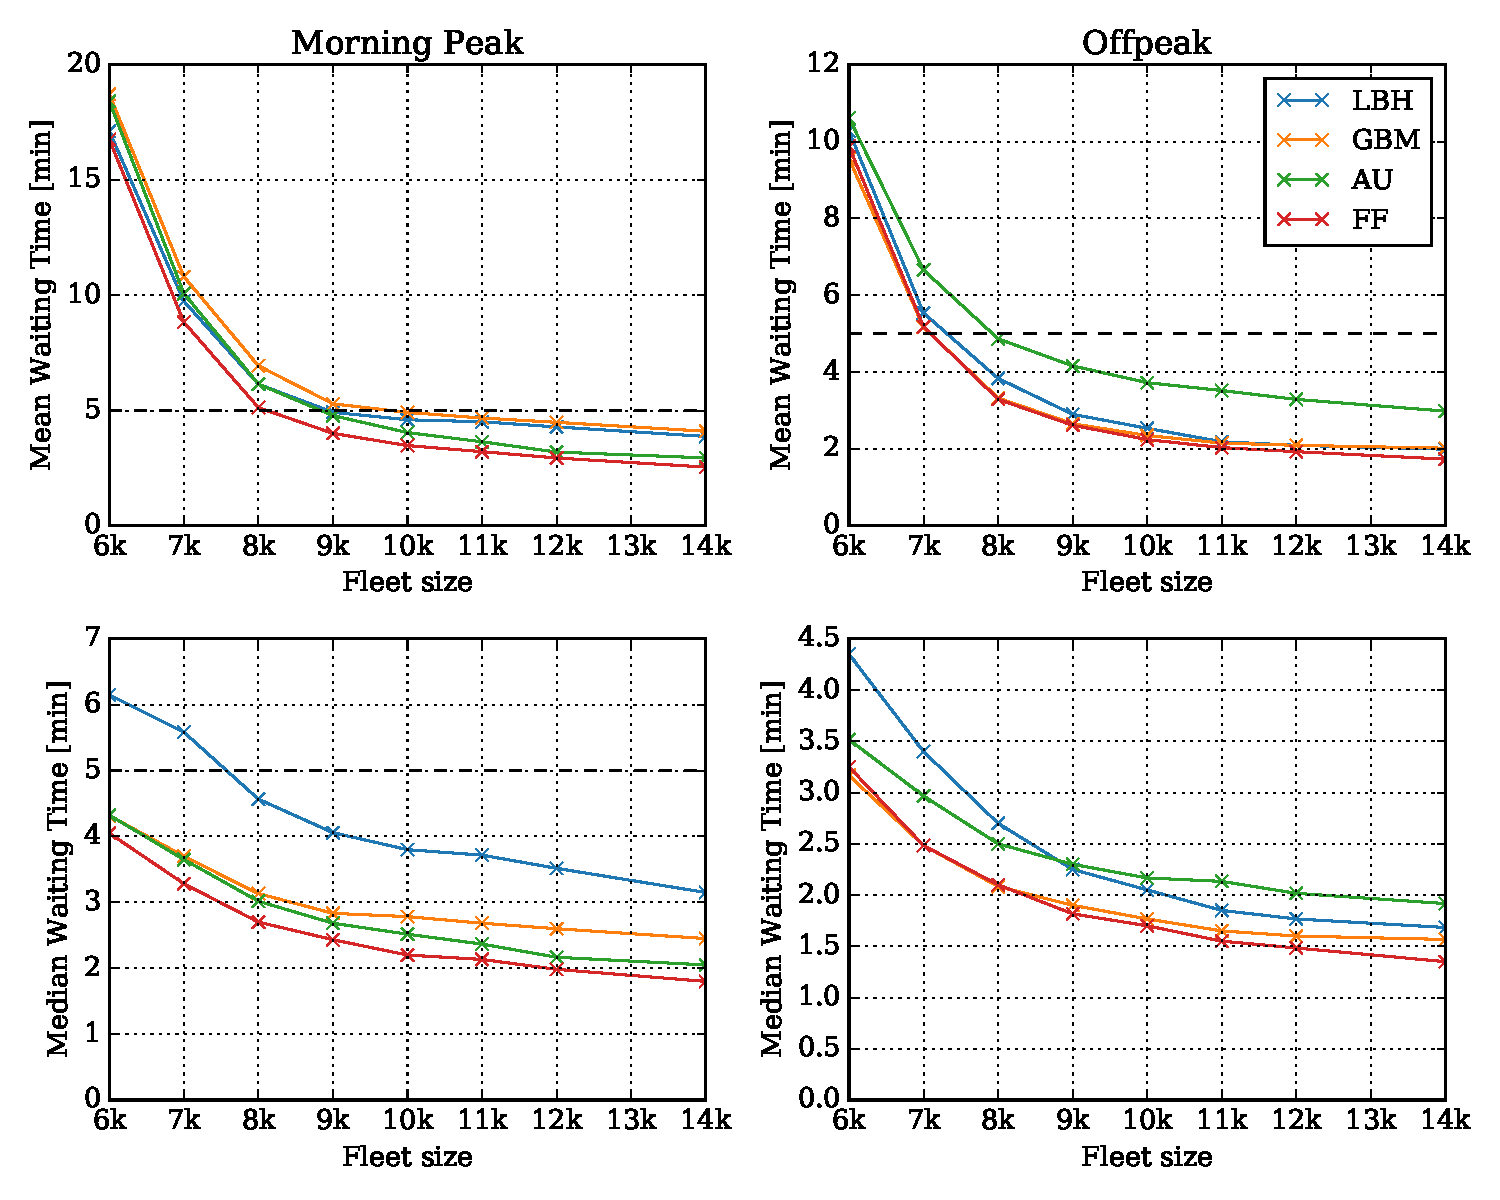
\includegraphics[width=1.0\textwidth]{figures/waiting_times.pdf}
%    \caption{Comparison of mean/median peak/offpeak wait times for the four \sout{control algorithms}\hl{operational policies}\hl{ , I would describe the lines in this plot}}
%    \label{fig:waiting_times}
%\end{figure}

For Zurich, the times with peak congestion and, hence, longest travel times are from 6:30 to 9:00 am and from 4:30 pm to 6:30pm. Figure \ref{fig:wait_time} shows the 90\% quantile and mean wait times produced by different fleet sizes and operational policies for the morning peak (left) and for off-peak hours (11am - 3pm, right). As expected, the FF algorithm performs best, because it operates on a very detailed demand estimate and thus can anticipate trips better than any other algorithm. Interesting differences can be seen for the other algorithms; which produces the longest wait times depends strongly on the given use case. At peak times, the GBM algorithm produces the worst wait times, which can be explained by the fact that its only objective is the minimization of pickup distance. Hence, trips originating in remote areas will experience long wait times. For off-peak hours, the uniform rebalancer (AU) yields the longest wait times, because the uniform distribution of vehicles does not correspond to the rather segregated demand.
 

If one assumes that a wait time of 5 minutes at peak times is acceptable in 90\% of the cases (top left graph), one could reach this objective with fleet sizes of around 7,000 vehicles (FF) and 14,000 vehicles (GBM) in Zurich. The results also show that such fleet sizes would produce even lower wait times of around two to four minutes at off-peak times. Note that the choice of operating policy makes a difference in fleet size of up to 7000 vehicles here.


\subsection{Fleet Utilization}
\label{sec:cost_analysis}

%\begin{figure}
%    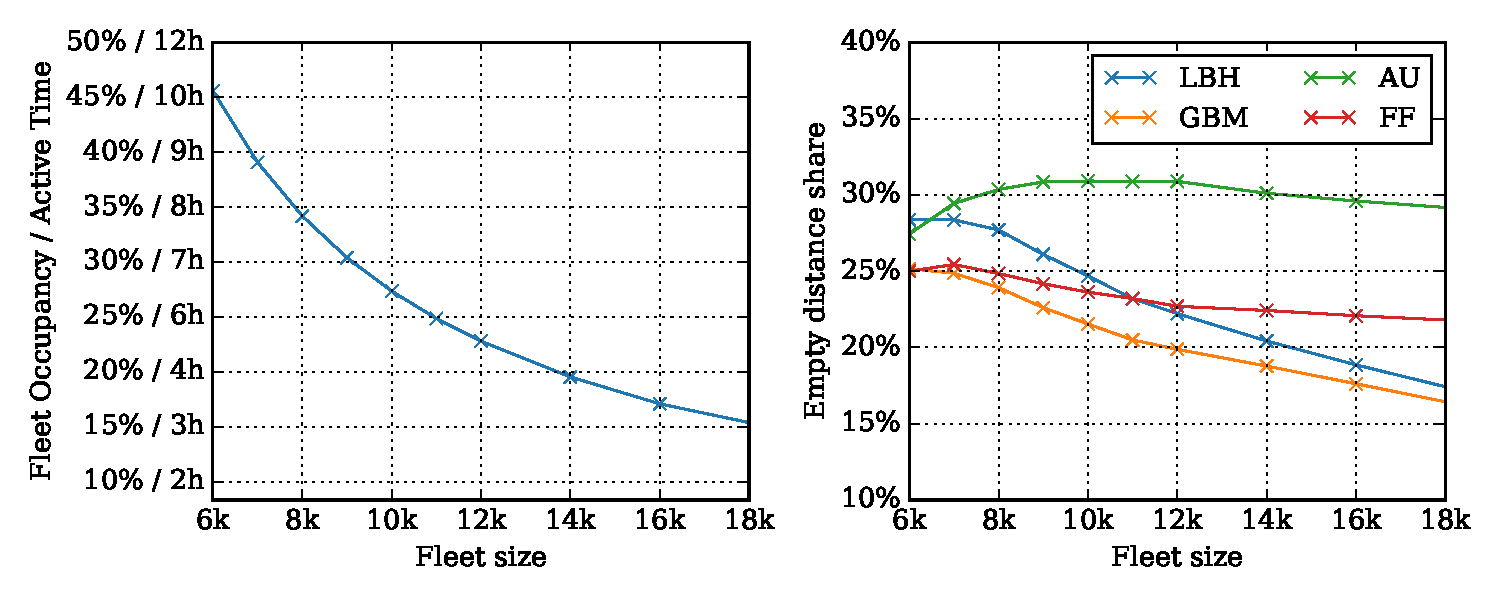
\includegraphics[width=1.0\textwidth]{figures/ratios.pdf}
%    \caption{Fleet occupancy (share of non-idle time) and share of empty distance for the four \sout{control algorithms}\hl{operational policies}  \hl{ I would make this plot bigger.}}
%    \label{fig:ratios}
%\end{figure}

\begin{figure}
\centering
\begin{subfigure}{0.5\textwidth}
  \centering
  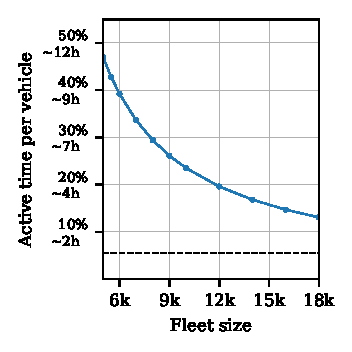
\includegraphics[width=2.35in]{figures/revision/rev_occupancy.pdf}
  %\caption{Fleet occupancy (active time)}
  %\label{fig:occupancy}
\end{subfigure}%
\begin{subfigure}{0.5\textwidth}
  \centering
  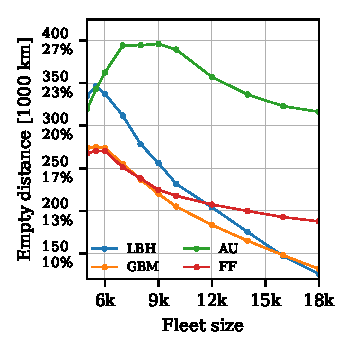
\includegraphics[width=2.35in]{figures/revision/rev_empty_miles.pdf}
  %\caption{Empty fleet distance}
  %\label{fig:empty_miles}
\end{subfigure}
\caption{Fleet performance metrics. Left: fleet occupancy or average active time of vehicles in the AMoD fleet. Right: empty distance produced by different operating policies. The percentage indicates the share of empty distance within total driven distance of the AMoD fleet.}
\label{fig:fleet_info}
\end{figure}

Two important metrics from the viewpoint of service profitability are the share of active hours (i.e. the time in which vehicles are actually occupied by a customer) and the share of empty distance.  Fleet occupancy is displayed in Figure \ref{fig:fleet_info} on the left. One can see that, with an increasing fleet size, occupancy declines. Occupancy times range from 9h per day with a fleet of 6,000 vehicles to only 3h a day with 18,000 vehicles. Occupancy times range from 9h per day with a fleet of 6,000 vehicles to only 3h a day with 18,000 vehicles. However, compared to the average usage times of private cars in Switzerland per day, which is 1.32h\citep{Bosch2016a}, one can see that, for any fleet size, vehicle utilization could increase by a factor of 2 to 7.


On the right, Figure \ref{fig:fleet_info} shows the share of empty distance driven by the AMoD fleets.Clearly, one can see how the objective of maintaining a uniform distribution of vehicles causes substantial empty distance for the AU algorithm. Also as expected, the GBM algorithm produces the least  empty distance - this is its sole objective. Furthermore it becomes evident that the rebalancing algorithms (AU and FF) have a lower sensitivity to increasing fleet sizes than the others, which is a direct consequence of rebalancing action. For the non-rebalancing algorithms, the probability that a vehicle is already there when a request pops up at any given location is increasing; thus, the empty distance ratio decreases rapidly. For the rebalancing algorithms, however, additional capacities in vehicle fleet are used to provide a better (according to the objective) balancing.


Looking at the actual distance driven by customers, it is possible to compare the amount of individual traffic (on the road) before the introduction of an AMoD fleet into the scenario and after (including the substituted public transport trips and empty distance). The increase of vehicle distance is about +25.5\% from 944,061 km to 1,184,795 km.

\subsection{Financial Analysis}
\label{sec:cost_analysis}

Based on the cost calculator for automated vehicle fleets in the Swiss context by \citet{Bosch2016a}, the costs of operating the AV services are computed based on key figures: occupancy, share of empty distance, operating times, trip lengths per passenger and average speed. In Figure~\ref{fig:financial} (left), the resulting price per (revenue) vehicle kilometer - including a profit margin of 3\% - is shown. One can observe that price increases with fleet size, which can be explained by lower occupancy rates. It should, however, also be pointed out that required price differs between the algorithms. The GBM algorithm generally operates at the lowest cost, because total distance driven by the fleet is minimized; the AU algorithm is most expensive, because of high empty distance as shown above. Nevertheless, direct comparison of prices at different fleet sizes shows that there are only slight differences between the algorithms.


The picture changes if one looks at the prices dependent on wait times for each policy as shown on the right side of Figure~\ref{fig:financial}. One can see that, out of the four proposed policies, the FF version is Pareto-optimal as it provides the shortest wait times in combination with the lowest prices. This does not come as a surprise, because the FF algorithm has full information about the demand patterns in the scenario. Second best, despite excessive rebalancing activity, is the AU policy for short wait times. Only from wait times of 7 minutes and more does it become cheaper to apply the non-rebalancing policies to achieve the same 90\% quantile wait times. Third is the simple heuristic approach, closely followed by the GBM policy.

%\begin{figure}
%    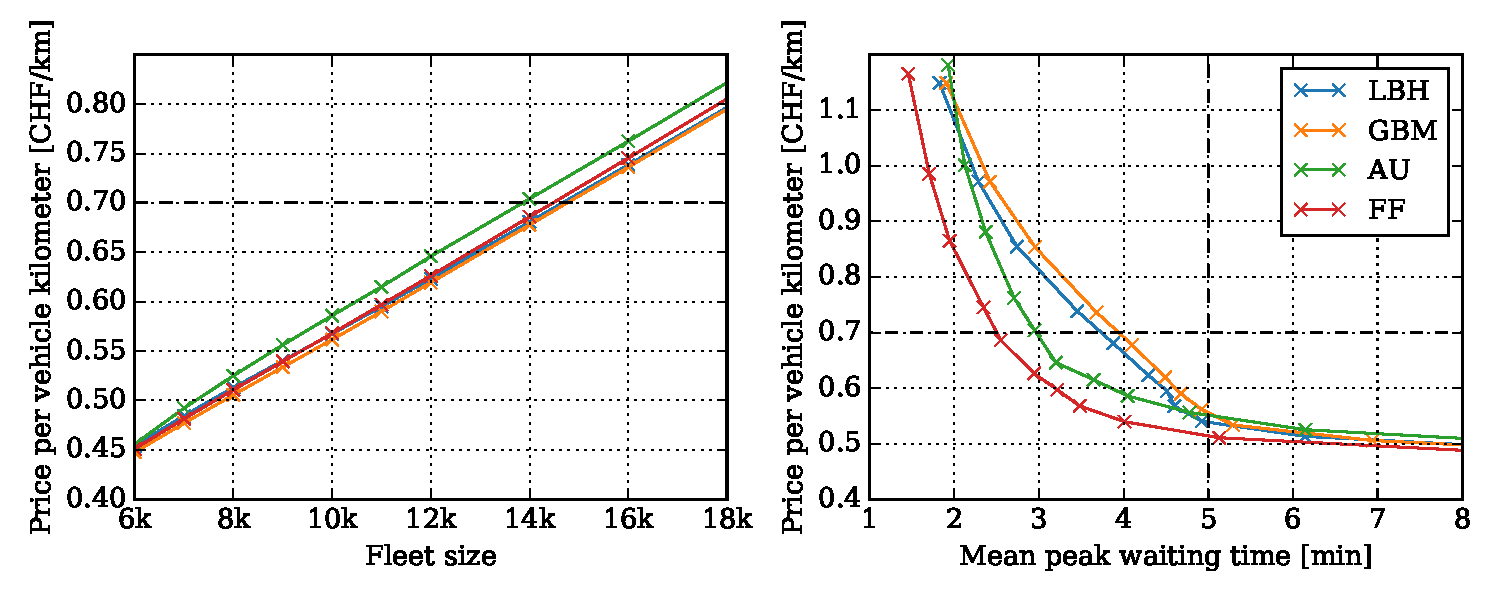
\includegraphics[width=1.0\textwidth]{figures/costs.pdf}
%    \caption{Cost analysis of the presented \sout{control algorithms}\hl{operational policies} \hl{ I would make this plot bigger.}}
%    \label{fig:costs}
%\end{figure}

\begin{figure}
\centering
\begin{subfigure}{0.5\textwidth}
  \centering
  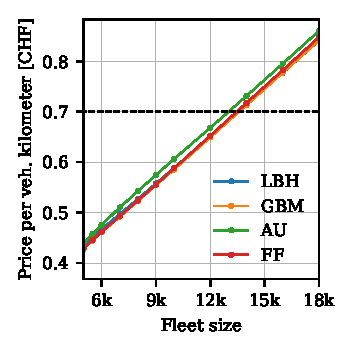
\includegraphics[width=2.35in]{figures/revision/rev_price.pdf}
%  \caption{}
%  \label{fig:cost}
\end{subfigure}%
\begin{subfigure}{0.5\textwidth}
  \centering
  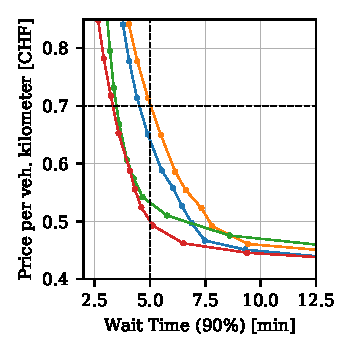
\includegraphics[width=2.35in]{figures/revision/rev_price_vs_waiting_time.pdf}
%  \caption{}
%  \label{fig:price_vs_waiting_time}
\end{subfigure}
\caption{Cost analysis of the presented policies. Left: cost per vehicle kilometer at given fleet sizes. Right: calculated costs in comparison to the achieved 90\% quantile morning peak wait times.}
\label{fig:financial}
\end{figure}




To allow for a more realistic comparison of the algorithms, we can define two boundaries: full costs for a private car in Switzerland are today estimated to be 0.7 CHF/km \citep{TCS2016}, which can be used as an upper bound for the price that customers would be willing to pay for the AMoD service. Furthermore, we can, again, assume that wait times should not be longer than 5 minutes. Given these two constraints (lower left quadrant in Figure~\ref{fig:financial}) we can see that algorithms with rebalancing have a clear advantage over those without. Ideally, looking at the FF algorithm, one could offer an AMoD service at 0.7 CHF/km if wait times of around 3.5 minutes are required during the morning peak, or one could offer the service for 0.5 CHF/km if wait times of 5 minutes are acceptable. Clearly, there is a  ``habitable zone'' for a fleet of automated taxis within those assumptions framed by fleet sizes of around 7,000 to 14,000 vehicles for the ideal FF dispatcher, which becomes even narrower for less optimal algorithms. Below those fleet sizes, wait times tend to get too high, while above that range the service becomes too expensive.


One can also see that under the given conditions (especially because the system operates at free-speed), a value of around 0.4 CHF/km constitutes a lower bound on the price of such an AMoD service. At significantly lower prices, it will not be possible to operate any service profitably.


\subsection{Costs in perspective}

To understand the attraction of the these AMoD services, it is necessary to compare prices with known figures for the city of Zurich\footnote{In 2017, one Swiss Franc (CHF) translated to approx. \$0.82 (USD) based on purchasing power parity  \citep{OECD2018}.}:
%\footnote{
%    \hl{In 2017, one Swiss Franc (CHF) translates to approx. \$0.82 (USD) based on purchasing power parity} \citep{OECD2018}.
%}:

Compared to taxi prices (base 8 CHF plus 5 CHF/km, \citet{StadtZurich2014}), the AV fleet is definitely much cheaper and potentially more convenient to use.However, the share of taxi use is rather low in Zurich; it seems unreasonable that an operator would deploy a fleet of a size suggested above just to capture this demand.


Variable costs for a private car in Switzerland are estimated to be 0.26 CHF/km \citep{TCS2016}, which is about half the minimium AMoD price specified above. This means that, for short term decisions, the fleet can not compete against private cars. Another important factor would be how highly people value spending time in automated taxis rather than driving their own car themselves. If autonomous vehicles are available, is it worth buying one’s own, private self-driving car? Another important thought: shared automated vehicles allow substantial freedom and independence, unlike classic car ownership. As shown above, using an AMoD fleet is substantially cheaper than the full costs of owning a private car (0.7 CHF/km). In that sense, the transition from vehicle ownership to the sharing economy may be the biggest motivating factor for the adoption of automated vehicles.


AMoD services are not competitive with (subsidized) public transport, for which users spend around 0.25 CHF/km  \citep{Bosch2016a}.Again, there are additional factors to consider, like greater service flexibility and lack of walks to transit stops. Another interesting question arises if one considers the unsubsidized costs of the public transit system, which could be up to 0.5 CHF/km. With that number, the figures could even become interesting for public transit operators to contemplate replacing conventional (unprofitable) lines with automated taxis - a concept that was explored further in  \cite{trainPaper} for rural train lines in Switzerland.

\subsection{Applicability to reality} 

The simulations use the full set of all requests that would occur during one day in Zurich city in a maximum demand scenario. It is thus interesting to have a look at run times of such simulations, especially because linear programs are run repeatedly during the simulation.


To compare, a run time of 35 minutes has been measured for the base simulation without any AMoD services and fleet management logic. The introduction of those components still leads to a run time of under 1h for most combinations of fleet sizes. Only the AU policy scaled rather strongly with fleet size, leading to simulation times of up to four hours. Hence, the optimizing algorithms are at least 6 times faster than would be necessary to operate in real time. In practice, algorithms could therefore either be run with shorter planning horizons (given that those don’t worsen the outcomes), or substantially more complex algorithms could be used.